\documentclass{article}
\usepackage{ctex}
\usepackage{graphicx}
\usepackage{amsmath}
\usepackage{indentfirst}
\usepackage{titlesec}
\usepackage{setspace}
\usepackage{subfigure}
\usepackage{caption}
\usepackage{float}
\usepackage{booktabs}
\usepackage{geometry}
\usepackage{multirow}
\geometry{left=1.2cm,right=1.2cm,top=2cm,bottom=2cm}
\title{\songti \zihao{2}\bfseries 红外荧光光谱实验报告}
\titleformat*{\section}{\songti\zihao{4}\bfseries}
\titleformat*{\subsection}{\songti\zihao{5}\bfseries}
\renewcommand\thesection{\arabic{section}}
\author{王启骅 PB20020580}
\begin{document}
	\maketitle
	\section{实验数据与分析}
	\subsection{稀土材料测量}
	\begin{figure}[!h]
		\centering
		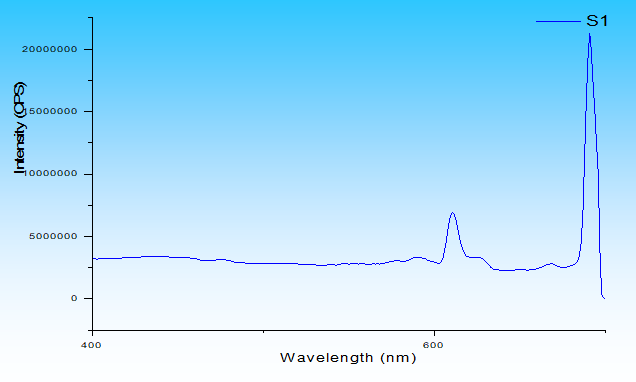
\includegraphics[scale=0.8]{1}
		\captionsetup{font={small},labelfont=bf}
		\caption{\heiti\zihao{-5}350nm粗测稀土材料荧光发射波长}
		
	\end{figure}


	\begin{figure}[!h]
	\centering
	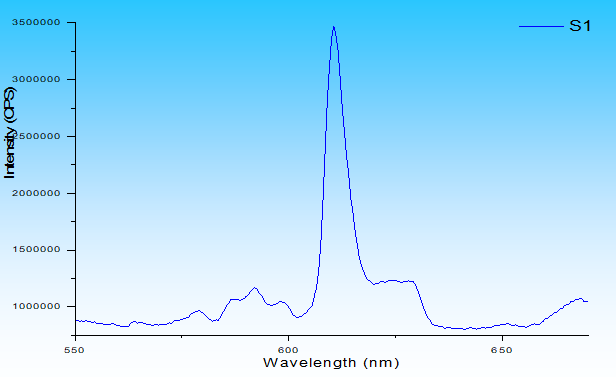
\includegraphics[scale=0.8]{2}
	\captionsetup{font={small},labelfont=bf}
	\caption{\heiti\zihao{-5}350nm在荧光波长附近测稀土材料}
	
\end{figure}
首先使用350nm波长的光粗测样品,这里采用360nm的滤光片,滤去入射光。测量从400nm到700nm的可见光波段步长1nm缝宽5mm,得到结果如图1所示。可见有两个峰,在610nm与700nm处,由于倍频效应,700nm的光来自于激发入射光350nm在样品上的反射,需要舍去,荧光在610nm附近。


我们进一步选取550nm到670nm处进行细测,步长0.5nm,并减小缝宽到3mm提高分辨率,得到如图2所示。
	
	
	接下来测样品的激发波长,如图3三幅图分别为荧光/激发光,荧光绝对强度,激发光绝对强度。激发光在260-600nm步长1nm缝宽5mm,测荧光610nm时的以上强度。可以看出虽然在约400nm和460nm处荧光强度较高,但事实上此时激发光的强度也很高,导致归一化后的相对强度只有很小的峰。由于对同一波长,荧光强度$ \propto $激发光强度,则我们需要选取相对强度最高的波长,即260nm为合适的荧光激发波长。
		\begin{figure}[!h]
		\centering
		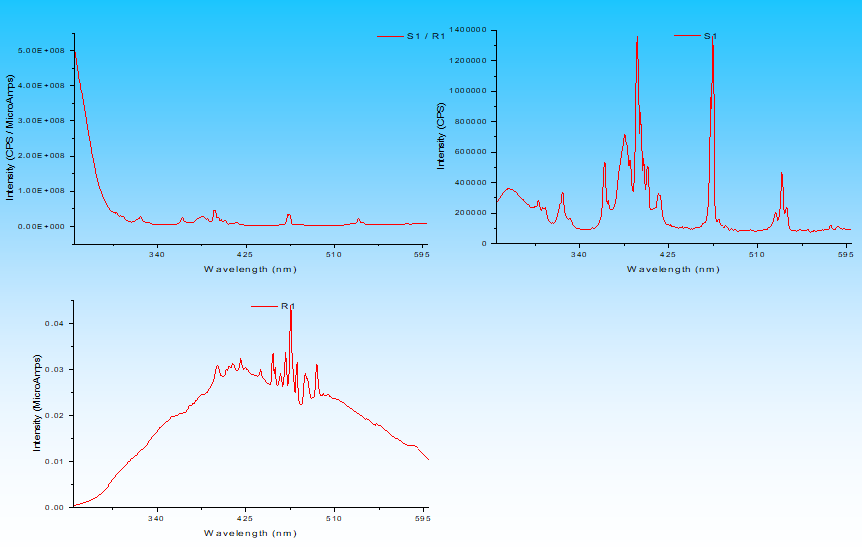
\includegraphics[scale=0.8]{EX1}
		\captionsetup{font={small},labelfont=bf}
		\caption{\heiti\zihao{-5}稀土材料荧光激发波长测量}
		
	\end{figure}


	\begin{figure}[!h]
	\centering
	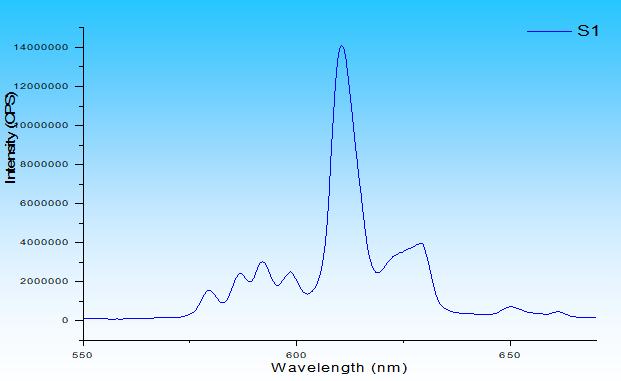
\includegraphics[scale=0.8]{3}
	\captionsetup{font={small},labelfont=bf}
	\caption{\heiti\zihao{-5}260nm稀土材料荧光发射波长}
	
\end{figure}



设置激发光波长260nm,以相同的方法测量550-670nm荧光,步长0.5nm,缝宽3mm,得到如图4。根据图2,3,4可见在入射光强减弱下,260nm对应的荧光强度明显增强。


	
	\subsection{有机样品测量}

首先使用350nm波长的光粗测样品,这里采用360nm的滤光片。测量从400nm到700nm的可见光波段步长1nm缝宽5mm,得到结果如图1所示。可见有单峰,在590nm。
		\begin{figure}[!h]
		\centering
		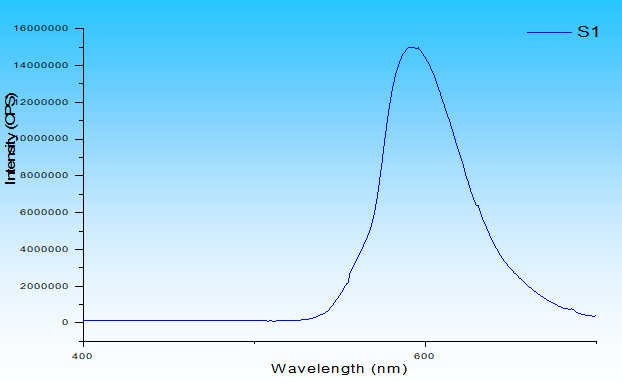
\includegraphics[scale=0.8]{4}
		\captionsetup{font={small},labelfont=bf}
		\caption{\heiti\zihao{-5}350nm粗测有机样品荧光发射波长}
		
	\end{figure}
	
	
	我们进一步选取500nm到700nm处进行细测,步长0.5nm,并减小缝宽到3mm提高分辨率,得到如图2所示。
	\begin{figure}[!h]
		\centering
		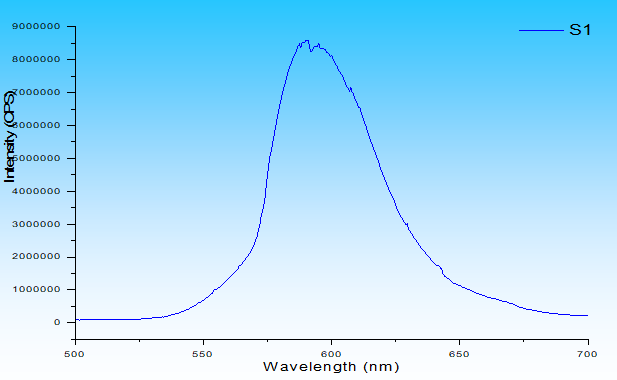
\includegraphics[scale=0.8]{5}
		\captionsetup{font={small},labelfont=bf}
		\caption{\heiti\zihao{-5}350nm在荧光波长附近测有机样品}
		
	\end{figure}
	
	
	接下来测样品的激发波长,如图3三幅图分别为荧光/激发光,荧光绝对强度,激发光绝对强度。激发光在260-550nm步长1nm缝宽5mm,测荧光590nm时的以上强度。可以看出荧光强度的变化趋势和激发光强度的变化趋势基本一致,所以荧光相对强度与激发光的波长并没有很大的联系。
	\begin{figure}[!h]
		\centering
		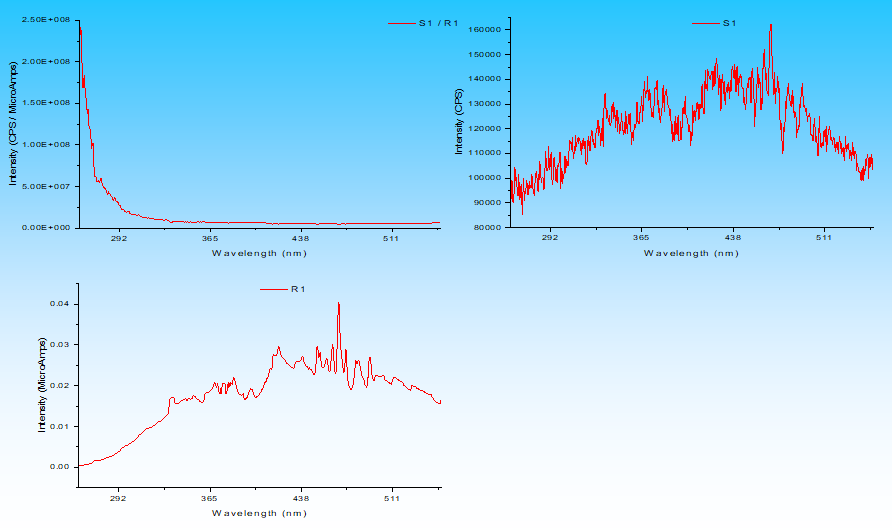
\includegraphics[scale=0.8]{EX2}
		\captionsetup{font={small},labelfont=bf}
		\caption{\heiti\zihao{-5}有机样品荧光激发波长测量}
		
	\end{figure}
	
	
	这也是为什么我们在图4设置入射激发光为260nm后,测量得到的荧光光谱结果反而较原来350nm结果光强更差,此时由于本身入射光强弱,导致对荧光测量产生影响。
	\begin{figure}[!h]
		\centering
		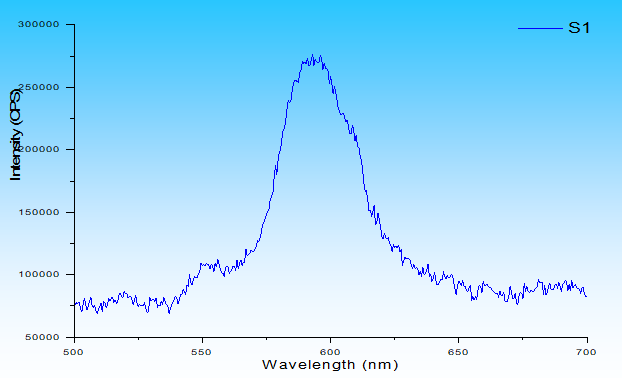
\includegraphics[scale=0.8]{6}
		\captionsetup{font={small},labelfont=bf}
		\caption{\heiti\zihao{-5}260nm有机样品荧光发射波长}
		
	\end{figure}


	对比稀土材料相对于有机材料,具有明显的单原子特征,即能谱较为锐利,且存在多个峰,能量取值高度量子化;而有机材料的荧光光谱峰则较为弥散,取值较为连续,具有明显的官能团特征(多个例子强耦合在一起,使能级分布连续)。差异来自于稀土材料因为其原子特征明显,其吸收光谱也具有高度的选择性,选取适当的发射光谱得到的发射强度会显著变大,而有机材料因为能级分布连续,选择性低,对任何波长的入射光具有相似的荧光发射强度。
	
	
	
	\section{思考题}
	\paragraph{1.}
	
	本次实验中用到的时JB510滤色片,为长波截止滤色片,在测量红外光谱时使用,放置于红外探测器前的发射单色仪前。
	
	
	本次实验没有用到ZWB2滤色片为短波截止滤色片,可以用于上转换荧光等荧光光子能量大于激发光的光谱的测量。
	
	
	\paragraph{2.}
	
	光栅为:
	$$
	d \sin{\theta}= m \lambda \qquad m=0,\pm 1,\pm 2 \dots
	$$
	其中 $d$ 为光栅常数,分别为:
	$$
	d_1=\frac{1}{1200}mm \approx 833nm \qquad d_2=\frac{1}{600}mm \approx 1667nm
	$$
	得到波长:
	$$
	\lambda_1=\frac{d_1}{m} = \frac{833}{m} nm \qquad m=1,2,3 \dots 
	$$
	$$
	\lambda_2=\frac{d_2}{m} = \frac{1667}{m} nm \qquad m=1,2,3 \dots 
	$$
	因此第一块是可见光栅,第二块为红外光栅。
	
	光栅的色分辨本领为:
	$$
	R=mN=m\frac{D}{d}
	$$
	其中,$D$ 为光栅的尺寸,$d$ 为光栅常数。因此,对于相同大小的光栅,刻槽密度 $1200条/mm$ 的光栅分辨率较高。
	
	\paragraph{3.}
	
		(1)	提高入射激发的光强(在不考虑成本下)。
		
		
		(2)	提高激发光的单色性。
		
		
		(3)   使用更纯净的样品,除去杂质可能对峰的判断影响。
		
		
		(4)	选用合适的滤光片。
\end{document}